\section{Preventivo costi}

Ogni studente del gruppo si impegna a lavorare al progetto per un monte totale di 92 ore
produttive. Sulla base della precedente analisi è emersa la seguente distribuzione orari con il corrispondente prospetto economico:

\begin{table}[H]
    \centering
    \renewcommand{\arraystretch}{1.5}
    \arrayrulecolor{black} % Colore del bordo della tabella
    % Definiamo la colonna grigio chiaro per la prima e l'ultima colonna
    \begin{tabular}{|>{\bfseries}c|c|c|c|c|c|c|>{\bfseries}c|}
        \hline
        % Prima riga - Grigio molto scuro, testo bianco in grassetto
        \rowcolor{gray!70} 
        \color{white}\textbf{Ruolo} & \color{white}\textbf{Costo orario (\euro/h)} & \color{white}\textbf{Ore (h)} & \color{white}\textbf{Costo (\euro)} \\
        \hline
        % Righe alternate con bianco e grigio chiaro
        \color{black}\textbf{Responsabile} & 30 & 64 & 1920  \\ 
        \hline
        \rowcolor{gray!10} % Grigio molto chiaro per riga alternata
        \color{black}\textbf{Amministratore} & 20 & 54 & 1080 \\ 
        \hline
        \color{black}\textbf{Analista} & 25 & 71 & 1775  \\ 
        \hline
        \rowcolor{gray!10} % Grigio molto chiaro per riga alternata
        \color{black}\textbf{Progettista} & 25 & 125 & 3125  \\ 
        \hline
         \color{black}\textbf{Programmatore} & 15 & 170 & 2550 \\ 
        \hline
        \rowcolor{gray!10} % Grigio molto chiaro per riga alternata
        \color{black}\textbf{Verificatore} & 15 & 160 & 2400 \\ 
        \hline

        % Ultima riga - Grigio molto scuro, testo bianco in grassetto
        \rowcolor{gray!70} 
        \color{white}\textbf{Totale} & \color{white} & \color{white}644 &  \cellcolor{black}\color{white}\textbf{12850}  \\ 
        \hline
    \end{tabular}


\end{table}

\begin{figure}[H]
    \centering
    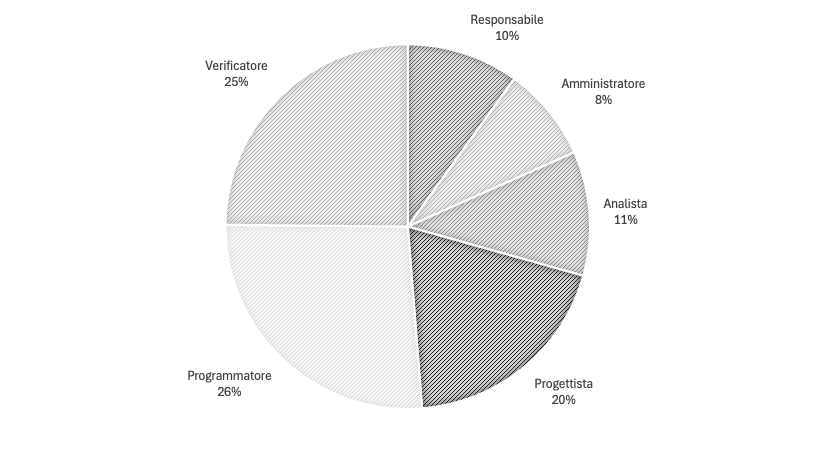
\includegraphics[width=\textwidth]{./images/piechart.png}
\end{figure}